\chapter{Coupling of Neuronal Model and Collective Dynamics}
    \section{Collective Behavior Experiments}
    The mechanisms that underly the dynamics of collective behavior as we observe it in many species like birds or fish have been of great interest.
    Theoretical work that has been developed to explain the observed behavior often relies on agent-based models with local interaction rules (\cite{Couzin2002}, \cite{Vicsek1995}).
    Recently, \cite{Strandburg-Peshkin2013} investigated the nature of these local interactions by performing an experiment with a fish school of 70 fish where a part of the group has been trained to move to a stimulus so that they could function as leaders of the group from which the information about the stimulus would spread during the experiment.
    By comparing different models to explain the spread of information in the group, which was approximated by the measured response times of the individuals, they found that a model that was based on visual input was supported the most by the observed data.\\
    In another experiment, \cite{Rosenthal2015} found that visual input also plays a crucial role in the spread of startle responses in a fish school.
    For this, they analyzed spontaneously occurring startle events in a fish school of roughly 150 golden shiners and looked at the factors that were most predictive of a fish to startle after the initial startle event.
    The two most predictive features that they found were the logarithmic distance to visible neighbors and the rank of subtended angular area of the initially startling fish on the retina of the focal fish \citep{Rosenthal2015}.
    Note, that due to the elongated body shape of the fish and the location of the eyes on the side, the subtended angular area is different from the distance alone because for example, a neighboring fish that is in front of the focal fish might be closer but it will cover a smaller part of the visual field than compared to a neighboring fish on the side.
    In the case of several neighbors, occlusions will also influence the ranking of the subtended angular areas.
    Based on these features \cite{Rosenthal2015} constructed an interaction network of the fish school and found that the local weighted clustering coefficient at the moment of an initial startle is informative of the size of the following cascade of startles.\\
    The first aspect of the startle behavior of the fish school that we were interested in was the frequency of spontaneously occurring startles.
    In the experiment of \cite{Rosenthal2015} the total number of 138 such startle events was acquired from recordings of 5 different groups over 53 minutes each so that the startling frequency of the group is around $8\cdot 10^{-3}$ startles per second and around $5\cdot 10^{-5}$ for an individual fish.
    A similar experiment that was done with 40 instead of 150 golden shiners found that the spontaneous startling frequency is around $5\cdot 10^{-4}$ to $1\cdot 10^{-3}$ for a single fish (Matt Grobis, Couzin Lab, private communication) and thus an order of magnitude higher than in the experiment of \cite{Rosenthal2015}.
    A possible explanation for the lower startling frequency in the bigger fish school might be a decreased responsiveness that is caused by the presence of other fish as it has been found in Guppies \citep{Fischer2015}.
    \section{Collective Behavior Model}\label{swarm_methods}
    In this section we will describe the model for the collective behavior, the integration of the neuronal model for the startle response initiation, the behavioral measurements and give an overview of the implementation.
	The model describes the individual motion of an agent by a stochastic differential equation that includes Brownian motion as described in \cite{Romanczuk2012a} and a continuous version of social interaction as described in \cite{Couzin2002}.
	We assume a set of $N$ interacting agents ($i= 1,\dots, N$).
	The dynamics of each agent in 2D is described by the following equations of motion:

	\begin{equation}
		\frac{d \vec{r}_i}{dt}=\vec{v}_i(t)
		\label{eq:r_diff}
	\end{equation}
	
	\begin{equation}
		\vec{v}_i(t) = {s_i\cos(\varphi_i(t)) \choose s_i\sin(\varphi_i(t)) }
		\label{eq:v_def}
	\end{equation}
	
	\begin{equation}
		\frac{d s_i}{dt} = \alpha\left( \mu_{s} - s_i\right) + F_{i, s} + \eta_{i, s}
		\label{eq:s_diff}
	\end{equation}
	
	\begin{equation}
		\frac{d \varphi_i}{dt} = \frac{1}{s_i + c_{s}}\left( F_{i,\varphi} + \eta_{i,\varphi} \right)
		\label{eq:phi_diff}
	\end{equation}
	
	Here $\vec{r}_i$ is the Cartesian position vector and $\vec{v}_i$ is the velocity vector, both of the focal agent.
	In the absence of social forces the speed $s_i$ of agent $i$ is relaxing towards the mean value $\mu_{s}$, which is the same for all agents, while we add the Gaussian white noise term $\eta_{i, s}$ and the relaxation time is determined by $\alpha$.
	The influence of the total effective social force is calculated by the projection onto the normalized velocity vector:
	
	\begin{equation}
		F_{i, s}=\vec{F}_i \cdot \vec{u}_{v, i} = \vec{F}_i { \cos\varphi_i \choose \sin\varphi_i }
		\label{eq:s_force}
	\end{equation}
	
	The change of direction $\varphi$ is mostly determined by $\vec{F}_{i,\varphi}$, the projection of the total effective social force onto the orthogonal of the normalized velocity vector and added Gaussian white noise represented by $\eta_{i,\varphi}$.
	
	\begin{equation}
		F_{i,\varphi}=\vec{F}_i \cdot \vec{u}_{\varphi,i} = \vec{F}_i {-\sin\varphi_i \choose \cos\varphi_i }
		\label{eq:phi_force}
	\end{equation}
	
	Additionally, we introduce the term $1/(s_i + c_s)$ to decrease the amount of direction change for high speeds where $c_s$ is meant to prevent numerical instabilities for very small $s_i$ values.
	The stochastic differential equations for the direction of motion of individual agents can be solved by a simple Euler-Maruyama method:
	
	\begin{equation}
		\varphi_i(t+1) = \varphi_i(t) + \frac{1}{s_i}\left( F_{i,\varphi}(t)\Delta t + \sqrt{2 \sigma_{\varphi}\Delta t} \text{ GRN(t)}\right)
		\label{eq:phi_update}
	\end{equation}
	
	\begin{equation}
		s_i(t+1) = s_i(t) + (\alpha (\mu_s - s_i(t)) + F_{i, s}(t))\Delta t + \sqrt{2 \sigma_{s} \Delta t} \text{ GRN(t)}
		\label{eq:s_update}
	\end{equation}
	
	\begin{equation}
		\vec{r}(t+1) = \vec{r}(t) + {s_i\cos(\varphi_i(t)) \choose s_i\sin(\varphi_i(t)) }
		\label{eq:r_update}
	\end{equation}
	Here "GRN(t)" is a Gaussian Random Number drawn from the standard normal distribution and $\sigma_\varphi$ and $\sigma_s$ are the standard deviations of direction and speed noise respectively.
	The total effective social force is a sum of three components:
	\begin{equation}
		\vec{F}_i=\vec{F}_{i,rep}+\vec{F}_{i,alg}+\vec{F}_{i,att}
		\label{eq:forces}
	\end{equation}
	Attraction:
	\begin{equation}
		\vec{F}_{i,att}= \frac{1}{n_{i,att}}\sum_{j \in Neigh} \mu_{att}S_{att}({r}_{ji}) \hat{r}_{ji}
		\label{eq:att}
	\end{equation}
	Repulsion:
	\begin{equation}
		\vec{F}_{i,rep}=\frac{1}{n_{i,rep}}\sum_{j \in Neigh} -\mu_{rep}S_{rep}({r}_{ji}) \hat{r}_{ji}
		\label{eq:rep}
	\end{equation}
	Alignment:
	\begin{equation}
		\vec{F}_{i,alg}=\frac{1}{n_{i,alg}}\sum_{j \in Neigh} \mu_{alg}S_{alg}({r}_{ji}) (\vec{v}_j-\vec{v}_i)
		\label{eq:alg}
	\end{equation}
	with $\vec{r}_{ji} = \vec{r}_j - \vec{r}_i$, $r_{ji} = |\vec{r}_{ji}|$ and $\hat r = \vec{r}/|r|$.
	Each component is computed by the normalized sum over the forces of the single interaction pairs with all agents of the neighborhood of the focal agent.
	For the metric interaction the neighborhood consists of all other agents and for the topological interaction the neighborhood consists of the Voronoi neighbors (for explanation, see Introduction).
	Note that the interaction range of the metric interaction is implemented by the weighting functions $S_X(r)$ that are sigmoid functions of distance, which go from 1 to 0, with the transition point at $r_{X,0}$ and steepness $a_{X}$:
	\begin{equation}
	S_X(r)=\frac{1}{2}\left(\tanh(-a_{X}(r-r_{X,0})+1\right)
	\label{eq:sigm}
	\end{equation}
	The strength of the different interactions is set by a constant $\mu_X$.
	For the normalization we use the number of effective neighbors $n_{i,X}$ which we define as the number of neighbors for topological interaction and for metric interaction we take the sum of the values of $S_X(r)$ so that $n_{i,X}$ will be approximately the number of agents within the interaction range:
	\begin{equation}
	n_{i,X} = \left\{\begin{array}{lc}
	|\{j, j \in Neigh\}|, & \text{for topological interaction}\\
	\sum_{j \in Neigh} S_X(r_{ji}), & \text{for metric interaction}
	\end{array}\right.
	\label{eq:neigh}
	\end{equation}\\
	Note, that due to numerical precision the numerical value returned by $S_X(r)$ is equal to zero for analytical values that are smaller than double precision which is in the order of $10^{-16}$.
	To avoid division by zero, we apply the normalization only for agents whose numerical value of $n_{i,X}$ is not zero.
	This also means that the ranges for the social forces are effectively longer since the normalization will rescale all non-zero values returned by $S_X(r)$ to the order of one.
	For the simulation of the fish school we define the basic time unit as seconds and the basic distance unit as one body length (BL) of a fish.
	We use a square arena of size $L$ with periodic boundaries so that the effective topology of the arena is a torus.
	\subsection{Coupling with neuronal model}
	For each agent we use the full neuronal model as described by equations \ref{eq:inhib} to \ref{eq:thrs} to initiate startle responses during the simulation.
    The resting activity of the inhibitory population $\rho_{0}$ of each agent was set to the mode of the fitted log-normal distribution from the previous chapter which was approximately $20.6$ in our case.
    For all other neuronal parameters we took the values that were either fixed or fitted in the previous chapter (see Table \ref{tab:neuroparams}).\\
    The last part that we need to define for the coupling is the visual input.
    In the previous chapter we had an abstract situation with only one stimulus but in the collective behavior simulations the agents are possibly surrounded by many neighbors.
    We considered three different methods to determine the effective visual input: max, k-nearest neighbors (KNN) and k-nearest mean deviate (KMD).
    For all methods we first computed the visual angle of each neighbor of the focal agent by assuming that the shape of an agent is a sphere with a diameter of one body length.
    Then, for the max method we simply took the maximal visual angle, i.e. the visual angle of the nearest neighbor.
    For the KNN method, we calculated the mean visual angle of the k nearest neighbors where k was fixed to the value 3.
    Finally, the KMD method is a combination of the former two methods where we subtracted the mean of the k nearest neighbors from the maximal visual angle.\\
    In the simulation these computations are performed at every time step to calculate the effective visual input for each agent.
    If this leads to a firing of the model M-cell of an agent we initiate a stereotypical startle response by replacing the total social force with a preset startle force:
	\begin{equation}
		\vec{F}_i =  {\mu_{st} \cos(\varphi_{st}) \choose \mu_{st} \sin(\varphi_{st})}.
		\label{eq:startle_force}
	\end{equation}
    Here, the amplitude $\mu_{st}$ was chosen to resemble experimentally measured accelerations and the escape direction $\varphi_{st}$ was drawn from the uniform distribution of the half circle that is pointing away from the direction of the mean distance vector to all agents, i.e. away from the group.
	\subsection{Behavioral Measurements}
	In order to analyze the behavior of the simulated fish school we measure 1) polarization, the degree to which the swimming directions are ordered, 2) cohesion, the degree to which the group stays together and 3) startling frequency, the average frequency of startles in the group.
	Other possible measurements that were not used due to limited scope of the project are the number and size of startle cascades where one startle response triggers a wave of subsequent startles and the mobility of the group, measured by the average traveled distance of the group.
	The group polarization is defined as the mean of the normalized velocity vectors for a given point in time:
	\begin{equation}
		p_{group}(t) = \frac{1}{N} \left| \sum_{i=1}^{N} \vec{v}_i(t) \right|
		\label{eq:pol}
	\end{equation}
	We define the cohesion in three different ways:
	\begin{equation}
		coh_{group}(t) = \left\{\begin{array}{lc}
		\frac{1}{N} \sum\limits_{i=1}^{N} \min\limits_{j \in Neigh} r_{ji}(t) , & \text{mean nearest neighbour distance}\\[12pt]
		\frac{1}{N} \sum\limits_{i=1}^{N}\frac{1}{N-1} \sum\limits_{j=1, j\neq i}^{N} r_{ji}(t), & \text{mean inter-individuell distance}\\[12pt]
		A(Conv(\{\vec{r}_i(t), i \in N \})), & \text{area of convex hull}
		\end{array}\right.
		\label{eq:coh}
	\end{equation}
	Here $A(Conv())$ denotes the area of the Convex Hull of the given set of points, i.e. the Cartesian positions of the agents at time $t$.
	If not noted otherwise, we used the mean nearest neighbor distance as the cohesion measure.
	The startling frequency is calculated for a full simulation run and simply the average number of startles per second.
	\subsection{Implementation}
	This project is based on an already existing implementation for the collective behavior with a different mechanism for the startle response initiation.
    All code can be found on the Github repository at \href{https://github.com/awakenting/master-thesis}{https://github.com/awakenting/master-thesis}.
	The model was implemented in Python 3.6 with the three main classes AgentData, BaseParams and AgentParams.
	An instance of AgentData contains all of the information about the agents that can change during the simulation or that can be different between individual agents and is thus the main data structure.
	The classes BaseParams and AgentParams contain fixed parameters of the simulated environment and global properties of the agents.\\
	In the main simulation function, for each time step, we first reset the social forces of each agent to zero, then we calculate the new social forces according to equations \ref{eq:att} to \ref{eq:alg}.
	Next, we update the inhibitory population activity and the membrane potential of all agents.
	For agents whose membrane potential reached the threshold we set the total force to the startle force as described by equation \ref{eq:startle_force} and for all others it is the sum of the three social forces as described by equation \ref{eq:forces}.
	Using the updated force the coordinates of the agents are finally updated according to equations \ref{eq:phi_update} to \ref{eq:r_update}.
    \section{Numerical experiments}
    In order to analyze the collective behavior model and its coupling with the neuronal model we chose most of the parameters such that the group behavior is comparable to the experiments mentioned earlier in this chapter.
    We fixed the number of agents to 40 and used a square arena with a side length of 40 BLs as in the experiments by Matt Grobis (Couzin Lab, private communication).
    Group behavior was simulated for a simulation time of 500 seconds.
    Most of the parameters of the collective model were fixed to values that are known to produce schooling behavior.
    Two parameters that we varied systematically were the mean speed of the agents $\mu_{s}$ and the noise on the direction change $\sigma_{\varphi}$ (referred to as "direction noise" in the following) as they allowed us to look at fish schools in different states in terms of polarization and cohesion.\\
    Our first measure of interest was the startling frequency.
    In Figure \ref{fig:swarm_heatmaps}, we see that except for the smallest mean speed, the startling frequency increases with increasing direction noise.
    There are also small increases in startling frequency for higher mean speed values but they are relatively low if compared to the effect of direction noise.
    The average nearest-neighbor distance shows the same pattern as the startling frequency with the highest values, i.e. the least cohesion, for highest speed as well as direction noise.
    In contrast, the mean polarization of the school over time is generally close to the possible maximal value and goes below $0.2$ only for the smallest speed and higher direction noise.
    Hence, it seems that a higher startling frequency leads to higher average nearest-neighbor distances.
    This is not true for the polarization where we find similar startling frequencies in the right-most columns of the heatmaps in Figure \ref{fig:swarm_heatmaps} but the mean polarization values range from 0.5 to 0.93.\\
    \begin{figure}[H]
    \begin{center}
    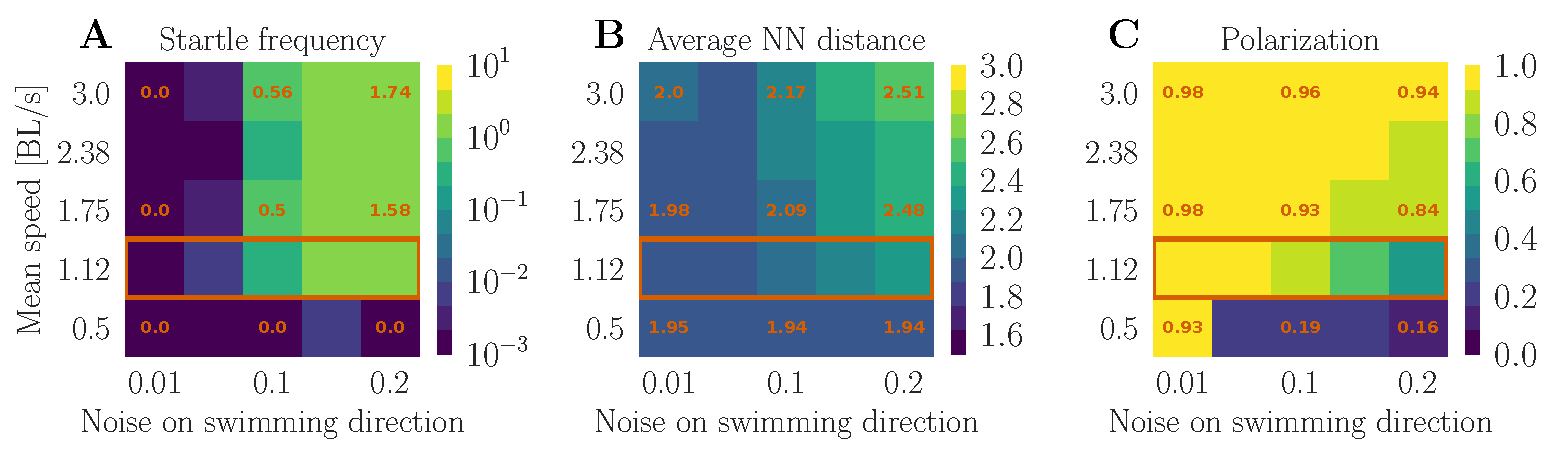
\includegraphics[width=\textwidth]{looming_swarm_fixed_rhonull_int_type_matrix_vis_method_knn_mean_deviate_new.pdf}
    \end{center}
    \caption{\textbf{Startle frequency dependency on collective properties.} Collective behavior results for metric interaction and with KNN-Mean-Deviate as visual integration method (see Section \ref{swarm_methods} for explanation). \textbf{A} Above a mean speed of 0.5 $BL/s$ the startle frequency only depends on the noise on the swimming direction of the individuals. It goes from no startles for very low noise to two startles per second for the highest noise that we analyzed here. \textbf{B} The average Nearest-Neighbor distance increases with noise on the swimming direction similar to the startle frequency but also increases with the mean speed in the range of higher noise values. \textbf{C} The polarization of the collective increases with the mean speed and decreases for higher noise on the swimming direction.}
    \label{fig:swarm_heatmaps}
    \end{figure}
    While we only looked at the mean values over time in Figure \ref{fig:swarm_heatmaps}, in Figure \ref{fig:swarm_over_time} we show how the different measures develop over time.
    For the case with medium direction noise level (left column in Figure \ref{fig:swarm_over_time}) we can clearly see how short periods with many startles affect the polarization as well as cohesion (see e.g. the time point at about 130 s).
    In the right column in Figure \ref{fig:swarm_over_time}, the high direction noise leads to fluctuations of higher amplitude for the polarization and cohesion.
    Additionally, the signals seem to undergo low-frequency oscillations with period lengths of around 60 s to 80 s which we also see for the lower direction noise but less pronounced.\\
    Next, we were interested in the spatial characteristics of single startle events.
    We restricted this analysis to simulations with a mean speed of 1.125 BL/s which is the second row from the bottom in the heatmaps in Figure \ref{fig:swarm_heatmaps}, also indicated by the orange box.
    Unfortunately, the simulations for a direction noise of 0.06 did not result in enough startle events so that we cannot properly analyze the results for this direction noise level.\\
    In the left column of Figure \ref{fig:swarm_startle_stats} we show the position of an agent at the time it startled.
    The coordinate system is build so that the center of mass of the school is at the origin and the mean movement direction of the school points upwards along the y-axis.
    At first glance, the startle positions are distributed similar to the positions of agents that did not startle although the startle positions tend to be more at the center of the school.
    This can be seen more clearly in the right column of Figure \ref{fig:swarm_startle_stats} where we show a histogram of the distance to the center of mass for startles and non-startles.
    Both histograms largely overlap but the startle distances are shifted by a small amount towards the center.
    The direction noise level does not change this pattern.\\
    In the last step of the spatial analysis, we measured the "frontness" of the startling agent by computing the mean movement direction of the group and projecting the position of the startling agent on the vector that originates from the center of mass of the group and points to the mean movement direction.
    The distribution of the frontness values for agents that do not startle (middle column in Figure \ref{fig:swarm_startle_stats}) is symmetric and Gaussian-shaped with the mean value at zero.
    The frontness values of the startling agents have a similar shaped distribution for a direction noise level of 0.1 but the distribution is more narrow which again indicates that the startle positions are closer to the center of the group.
    With increasing direction noise the distribution of startle frontness values becomes more skewed towards positive values, meaning that at high direction noise agents are more likely to startle when they are slightly more in the front than the average agent.\\
    We continue with a comparison of the different methods to determine the visual input of an agent.
    We focused so far on the KMD method where the visual input consists of the difference between the maximal visual angle and the mean of visual angles of the three nearest neighbors (as we fixed k=3).
    If we instead use the mean visual angle of the three nearest neighbors (KMEAN method) as the visual input the most salient difference is an increase of the startling frequency of about one order of magnitude (Figure \ref{fig:swarm_comparison}, left column, first row vs. second row. Note, that we used different colorbar scales in order to make the structure within the heatmaps visible).
    For the KMEAN method we also have startle activity for all combinations of the two parameters mean speed and direction noise which is not the case for the lowest direction noise in the KMD method.
    The effect of the direction noise is here dependent on the mean speed.
    While at higher speeds the startling frequency increases with higher direction noise as we observe it for KMD, at the lowest speed the startling frequency decreases for higher direction noise.
    The overall higher startling frequency is accompanied by nearest-neighbor distances that are up to twice as much as for the KMD method.
    Interestingly, the relationship between startling frequency and average nearest-neighbor distance is reversed for KMEAN because we find the highest nearest-neighbor distance for the lowest startling frequency.
    The polarization follows the same pattern as for KMD with a decrease of polarization for lower speed and for higher direction noise although the polarization does not decrease as much as in the KMD method.\\
    The differences between the MAX and KMD methods are in general similar to those just described for KMEAN.
    The startling frequencies are again much higher and even two to three times as high as for KMEAN.
    In contrast to KMEAN, the startling frequency always increases with increasing mean speed and increasing direction noise.
    Similar to KMEAN, the lowest startling frequency corresponds to the highest mean nearest-neighbor distance but in the case of MAX this point lies at the lowest mean speed and lowest direction noise.
    Finally, the polarization shows the same pattern as for KMD and KMEAN but it does not decrease as much so that the lowest value is at 0.56.    
    \begin{figure}[H]
    \begin{center}
    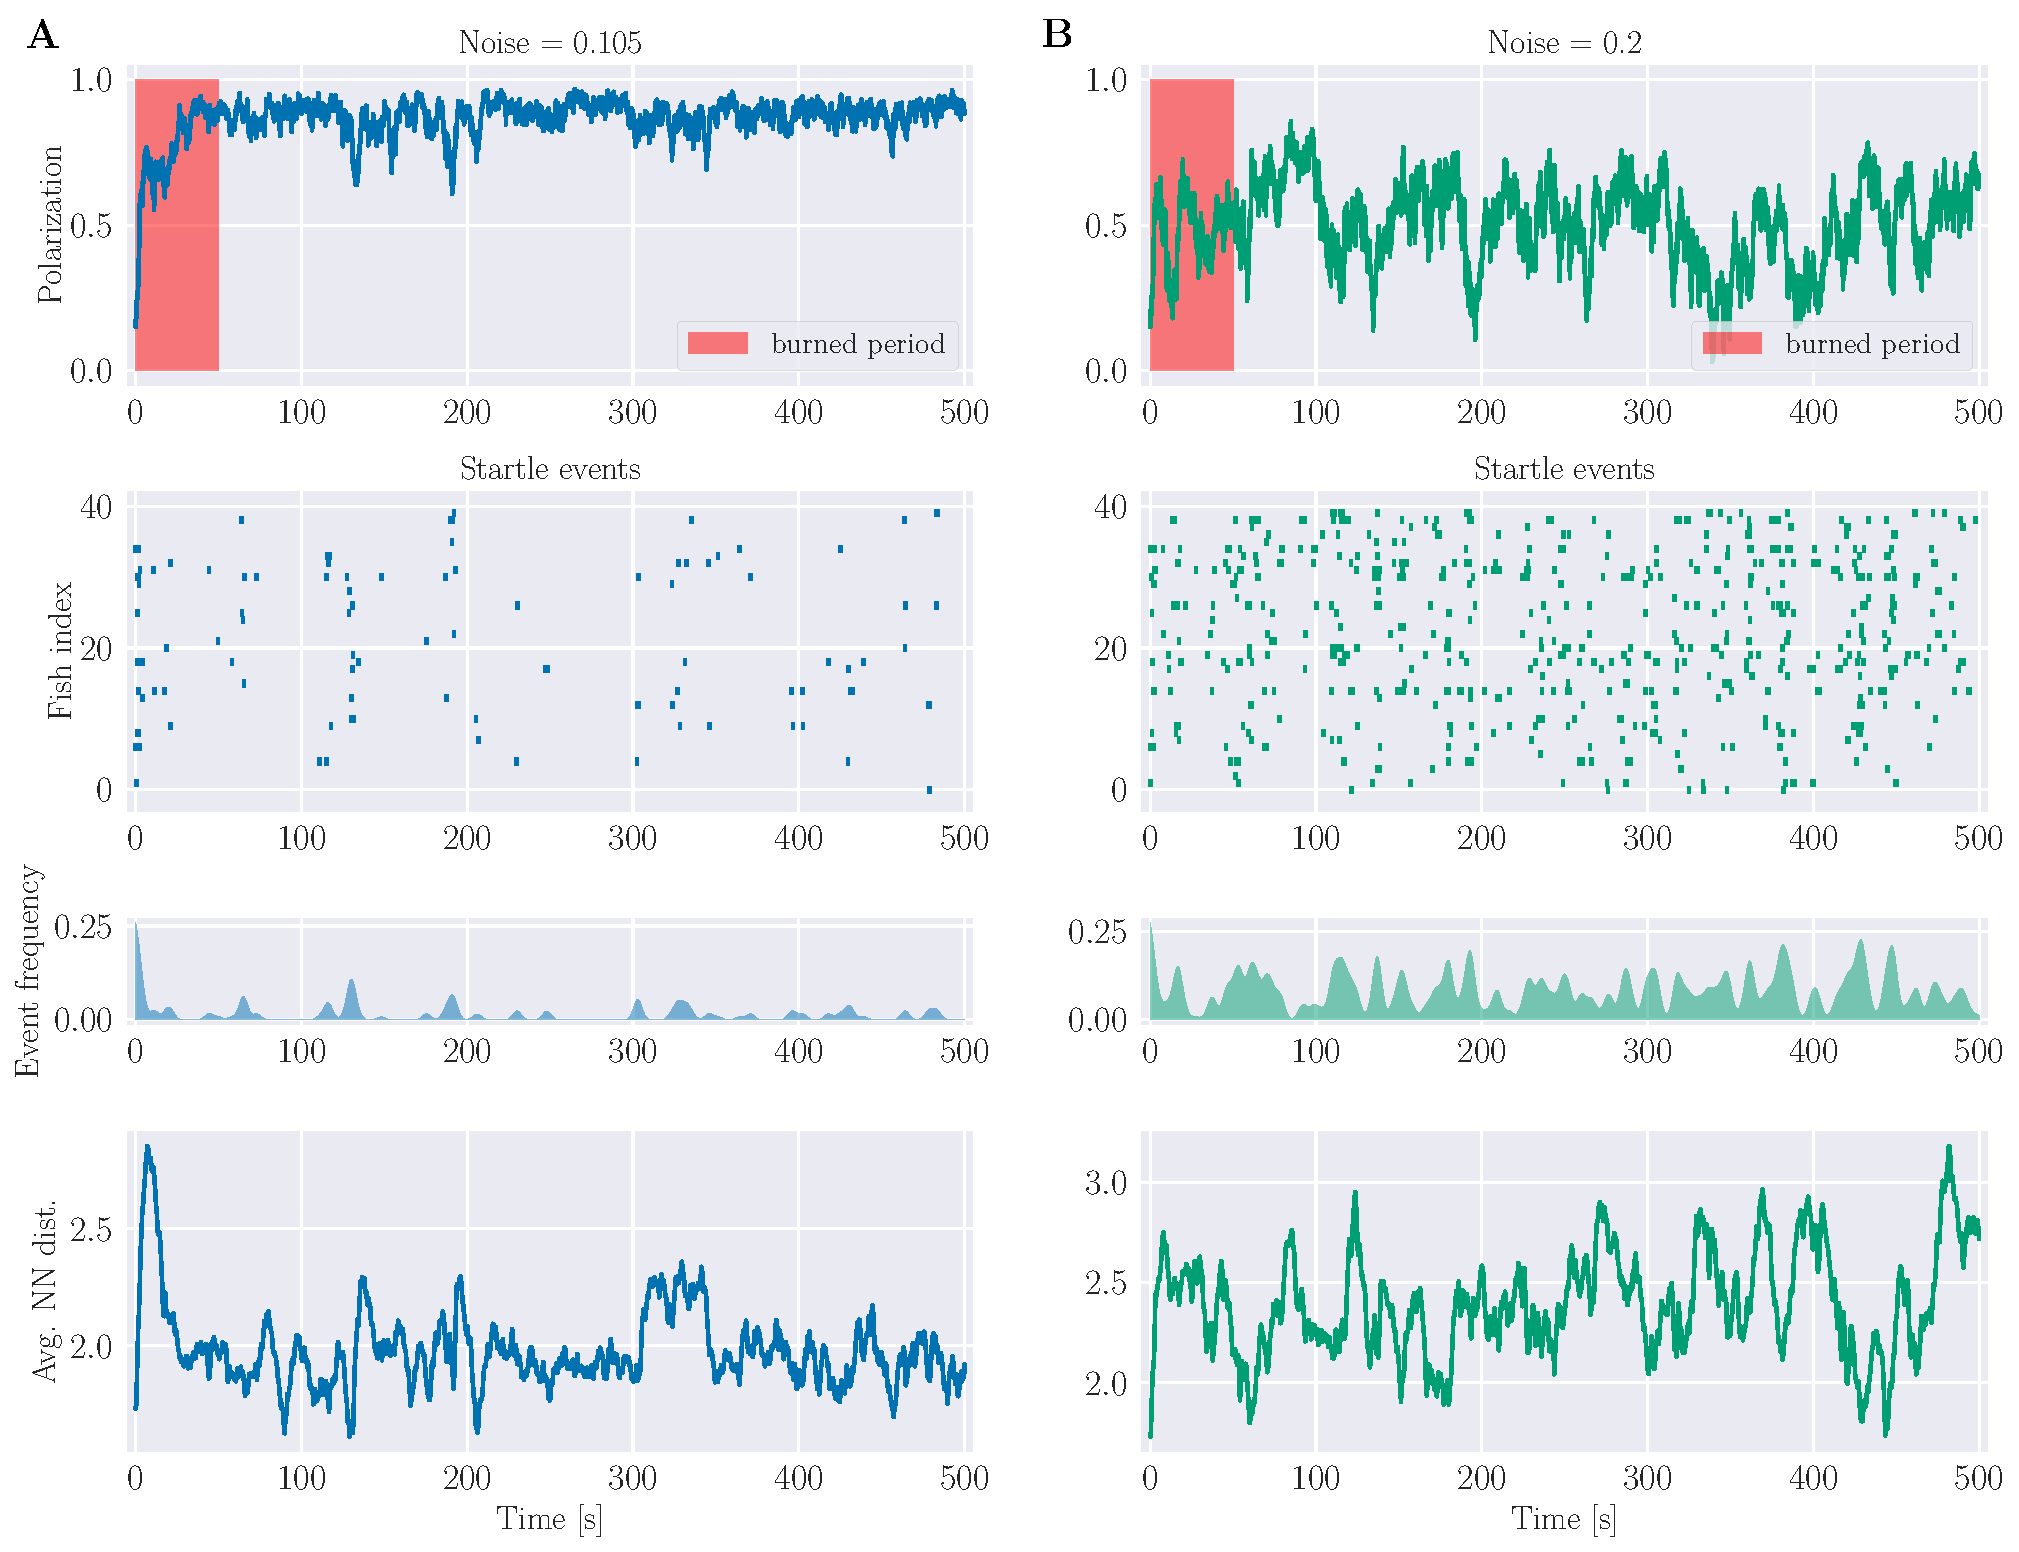
\includegraphics[width=\textwidth]{looming_swarm_over_time.pdf}
    \end{center}
    \caption{\textbf{Collective behavior properties over time for two examples.} The startling frequency, polarization and average nearest-neighbor distance are shown over time from two collective behavior simulations with metric interaction and with KNN-Mean-Deviate as visual integration method (see Section \ref{swarm_methods} for explanation). \textbf{A} For a medium swimming direction noise the polarization (top row) approaches a stable state 50 s after the simulation started. After many startle events in the initial time period the become more rare and come in short waves where many agents startle (second and third row). The group cohesion fluctuates around a value of 2 BL for the average nearest-neighbor distance. \textbf{B} For higher direction noise the polarization of the group shows high amplitude fluctuations around a mean value of 0.5. There are more startle events that seem to occur irregularly over time. The average nearest-neighbor distance shows similar to the polarization bigger fluctuations.}
    \label{fig:swarm_over_time}
    \end{figure}
    
    \begin{figure}[H]
    \begin{center}
    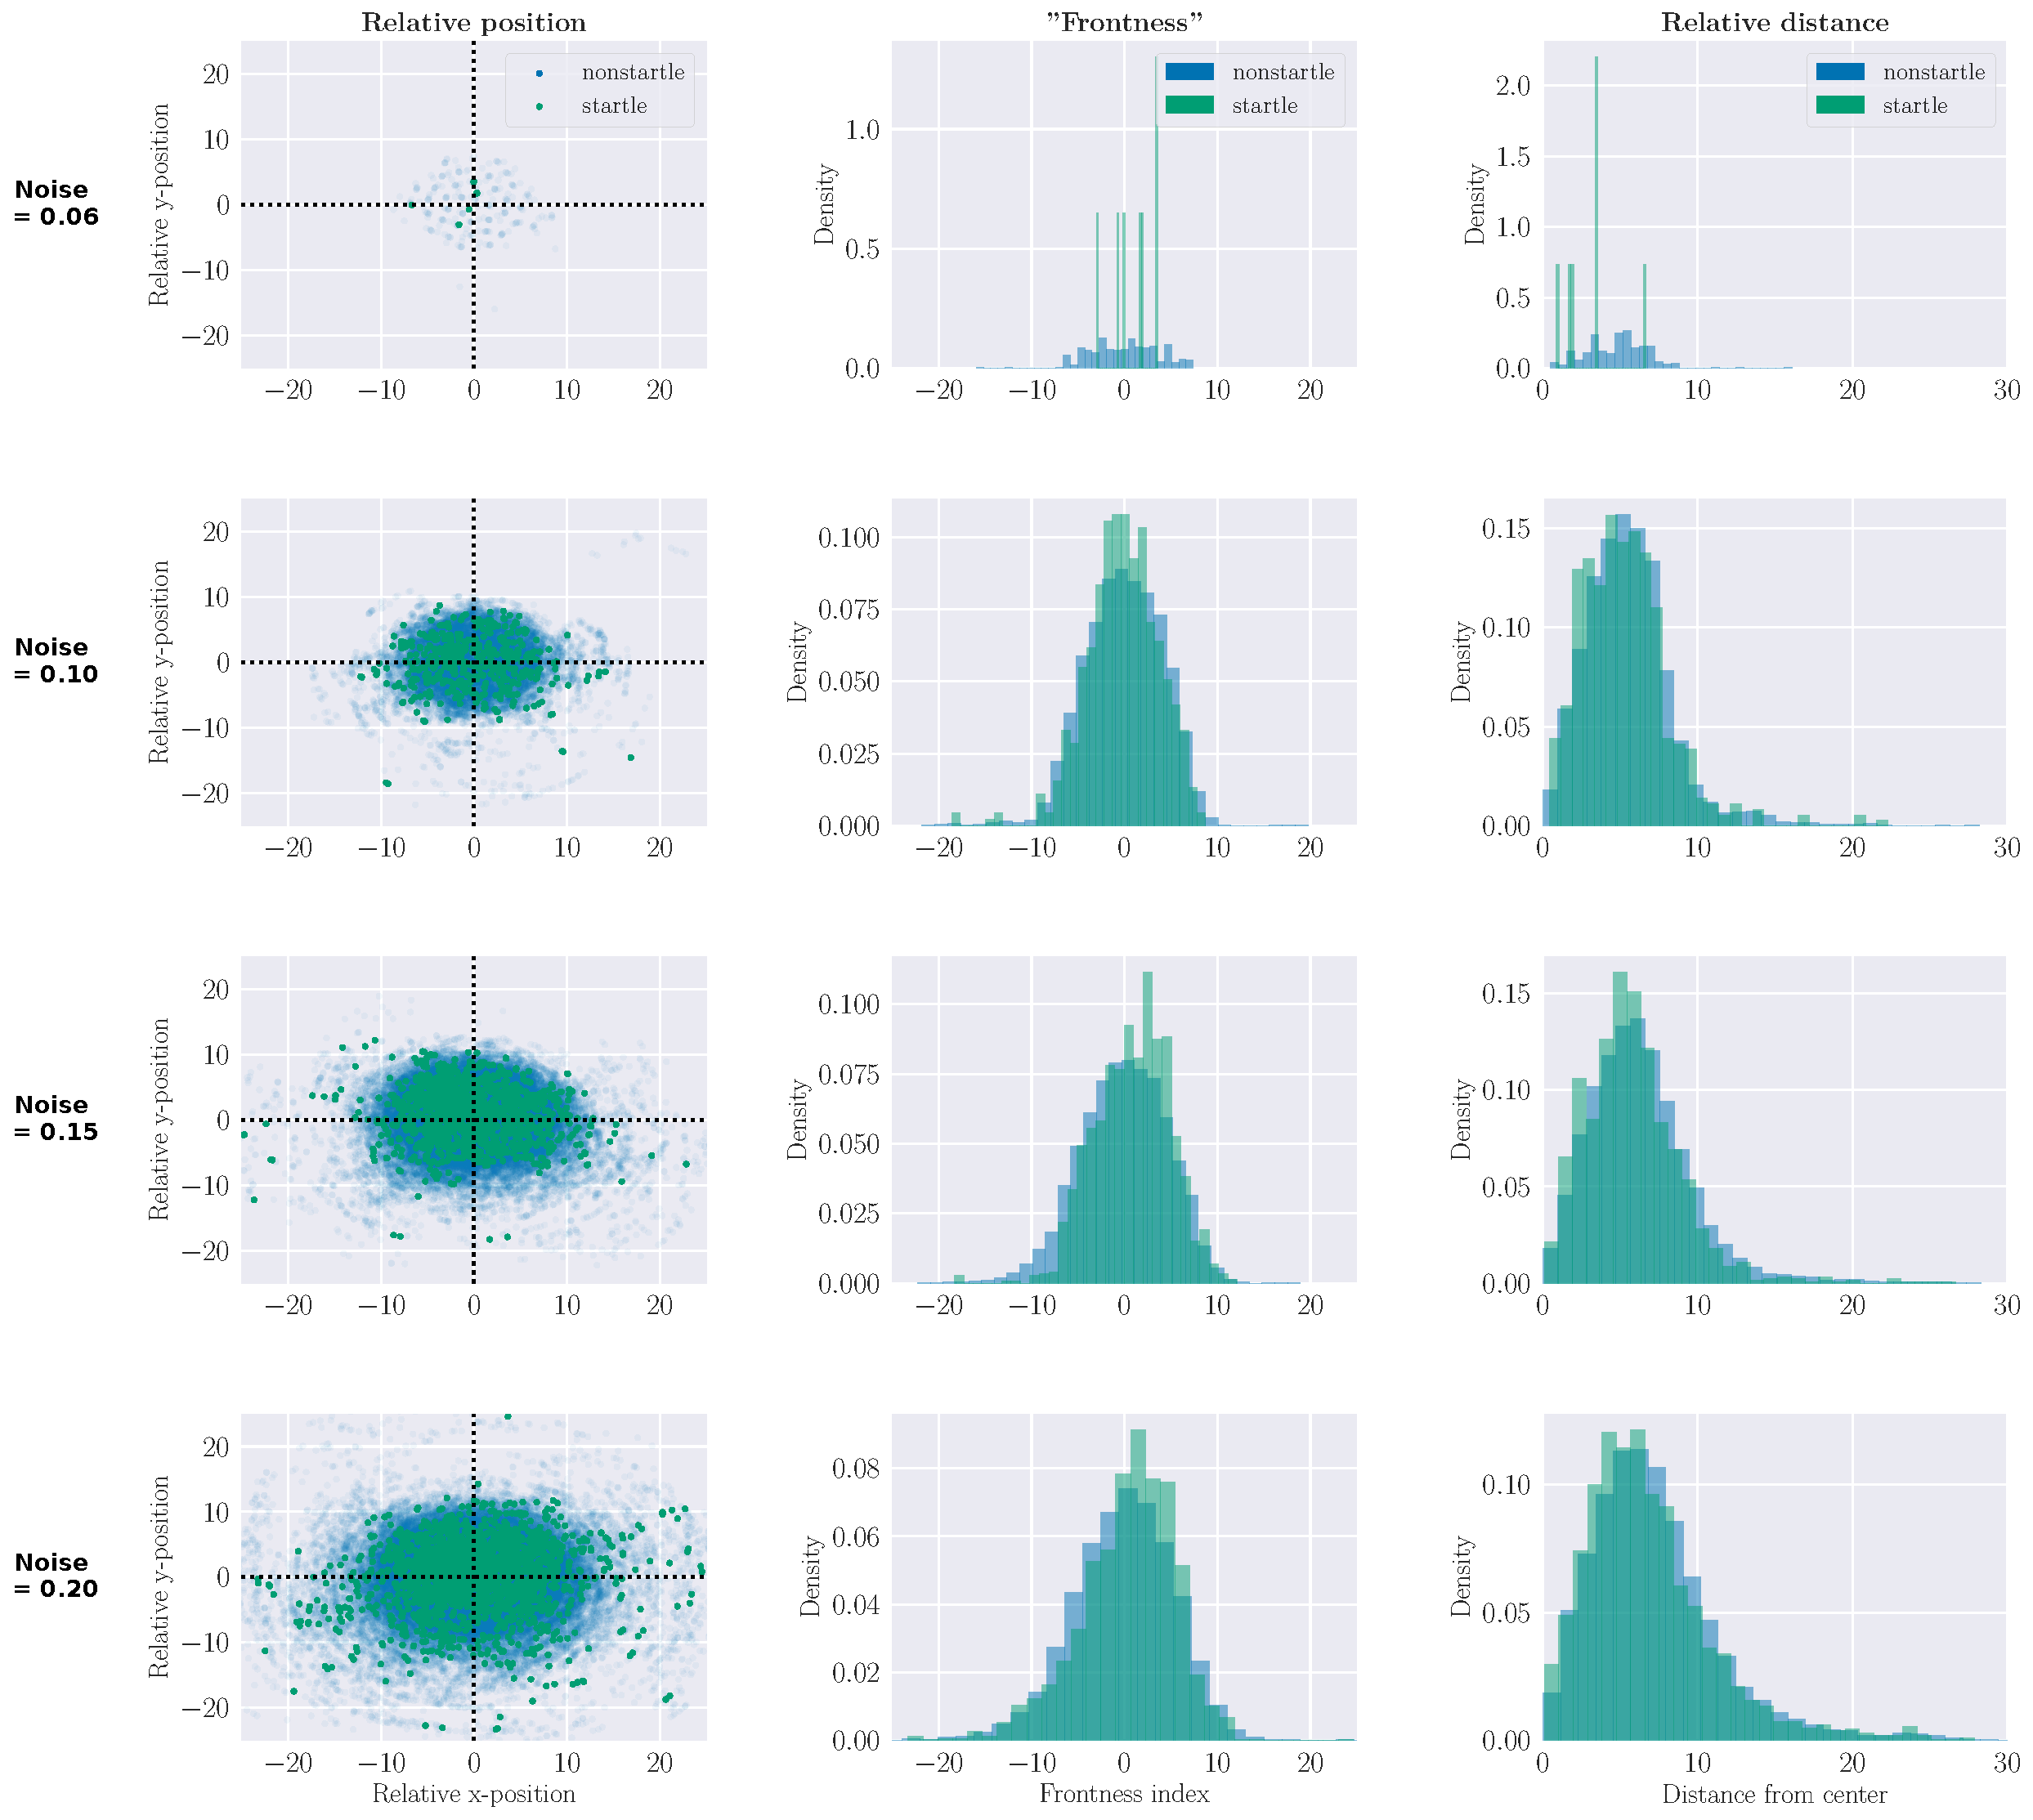
\includegraphics[width=\textwidth]{looming_swarm_startle_stats.pdf}
    \end{center}
    \caption{\textbf{School position at startle events.} Spatial properties of startle events for metric interaction and with KNN-Mean-Deviate as visual integration method (see Section \ref{swarm_methods} for explanation). Each row corresponds to a different direction noise value, starting with the smallest value for which the startle frequency was not zero at the top. The first columns shows for each startle event the relative position of the startling agent (green) and of all other agents (blue). The origin of the plot corresponds to the center of mass of the group and the mean direction in which the group is swimming is upwards along the y-axis. The second column shows the distribution of "frontness" values which is the the projection onto the vector that starts at the center of mass and points in the mean swimming direction of the school. The third column shows the distribution of the euclidean distance to the center of mass.}
    \label{fig:swarm_startle_stats}
    \end{figure}
    
    \begin{figure}[H]
    \begin{center}
    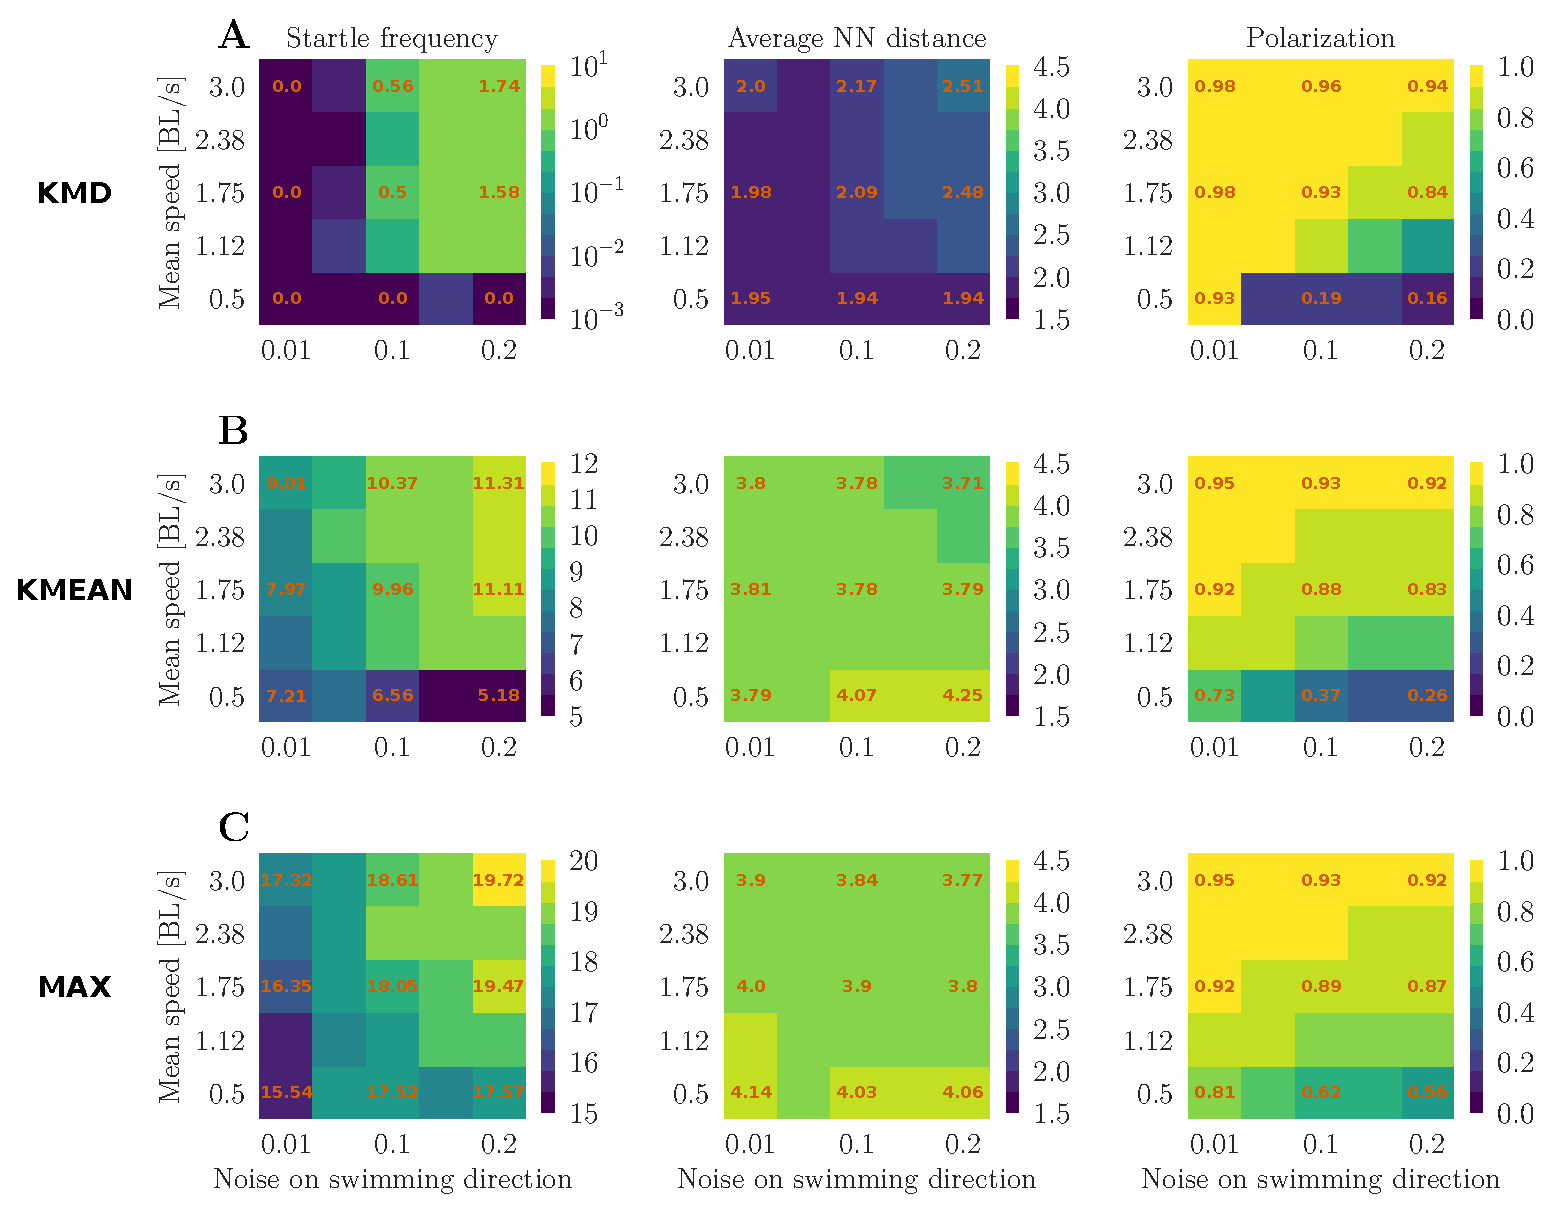
\includegraphics[width=\textwidth]{looming_swarm_fixed_rhonull_int_type_matrix_comparison_new.pdf}
    \end{center}
    \caption{\textbf{Comparison of different visual input methods.} Collective behavior results for metric interaction and different visual integration methods (see Section \ref{swarm_methods} for explanation). The same measurements as in Figure \ref{fig:swarm_heatmaps} are shown. \textbf{A} The same heatmaps as in Figure \ref{fig:swarm_heatmaps}, shown again here for better comparison. \textbf{B} The startle frequency, cohesion and polarization for the KMEAN method. The general patterns with respect to effects of mean speed and direction noise are similar to KMD although the startling frequency is much higher and the average nearest-neighbor distance is almost twice as big. \textbf{C} As for KMEAN, the general pattern is similar to KMD although the startling frequency is much higher for the MAX method.}
    \label{fig:swarm_comparison}
    \end{figure}
